\documentclass[12pt,letterpaper]{article}
\usepackage{fullpage}
\usepackage[top=1.5cm, bottom=3.5cm, left=2.2cm, right=2.2cm]{geometry}
\usepackage{amsmath,amsthm,amsfonts,amssymb,amscd, esint}
\usepackage{lastpage}
\usepackage{enumerate}
\usepackage{fancyhdr}
\usepackage{mathrsfs}
\usepackage{graphicx}
\usepackage{listings}
\usepackage{hyperref}
\usepackage[english]{babel}
\usepackage{lipsum}
\usepackage[table,xcdraw]{xcolor}
\usepackage{enumitem}
\usepackage{float}
\usepackage{chemfig}
\usepackage{yfonts}
\usepackage{tikz}
\usepackage{wrapfig}
\usepackage{url}
\usepackage{natbib}
\usepackage[normalem]{ulem}
\usepackage{multicol}
\useunder{\uline}{\ul}{}


%%%%%%%%%%%%%%% CODELISTINGS %%%%%%%%%%%%%%%%
\usepackage{listings}
\definecolor{codegreen}{rgb}{0,0.6,0}
\definecolor{codegray}{rgb}{0.5,0.5,0.5}
\definecolor{codepurple}{rgb}{0.58,0,0.82}
\definecolor{backcolour}{rgb}{0.95,0.95,0.92}

\lstdefinestyle{mystyle}{
    backgroundcolor=\color{backcolour},   
    commentstyle=\color{codegreen},
    keywordstyle=\color{magenta},
    numberstyle=\tiny\color{codegray},
    stringstyle=\color{codepurple},
    basicstyle=\ttfamily\footnotesize,
    breakatwhitespace=false,
    breaklines=true,                 
    captionpos=t,                    
    keepspaces=true,                 
    numbers=left,                    
    numbersep=5pt,                  
    showspaces=false,                
    showstringspaces=false,
    showtabs=false,                  
    tabsize=2
}

\lstset{style=mystyle}

%%%%%%%%%%%%%%%%%%%%%%%%%%%%%%%%%%%%%%% 
\usepackage{titlesec}
\usepackage{textcase} % for uppercase handling

% --- Section formatting ---
\titleformat{\section}
  {\normalfont\normalsize\bfseries\centering} % font size, bold, centered
  {\thesection}{1em}{\MakeTextUppercase} % uppercase text

% --- Subsection formatting ---
\titleformat{\subsection}
  {\normalfont\large\bfseries\centering}
  {\thesubsection}{1em}{\MakeTextUppercase}

% --- Roman numerals for numbering ---
\renewcommand{\thesection}{\Roman{section}}
\renewcommand{\thesubsection}{\Roman{section}.\roman{subsection}}

\newtheorem{definition}{Definition}
\newtheorem{observation}{Observation}
\newtheorem{reflection}{Reflection}
\newtheorem{PyPackage}{Package}
\newtheorem{book}{Book}

\newcommand{\HRule}[1]{\rule{\linewidth}{#1}}
\setcounter{tocdepth}{5}
\setcounter{secnumdepth}{5}

\setlength{\parindent}{0.0in}
\setlength{\parskip}{0.05in}

% Edit these as appropriate
\newcommand\course{}
\newcommand\subject{Final Degree Project}
\newcommand\degree{Bachelor's Degree in Physics}
\newcommand\documenttitle{Lower bounds of the success probability in quantum state exclusion for general ensembles}
\newcommand\NetIDb{Universitat Autònoma de Barcelona}
\newcommand\AuthorName{Sergio Castañeiras Morales}

\hypersetup{%
  pdftitle  = \documenttitle,
  pdfauthor = \AuthorName,
  pdfsubject= \degree,
  pdfcreator= \AuthorName,
}



\begin{document}
\title{\vspace{4cm} \normalsize 
		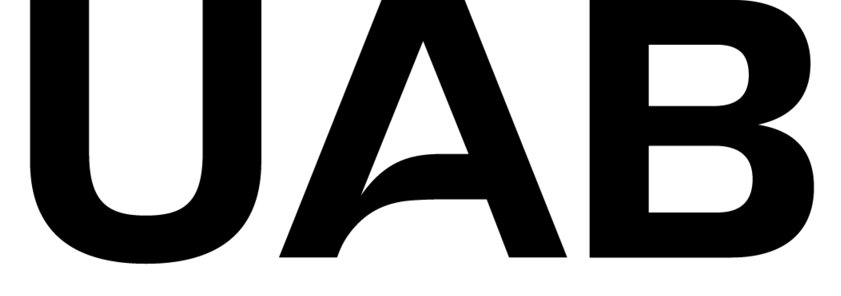
\includegraphics[width = 0.25\textwidth]{GeneralSources/UABLogo.png}\\ [0.5cm]
		\textsc{\NetIDb}\\ [2.0cm]
		\HRule{0.5pt} \\
		\LARGE \textbf{\uppercase{\documenttitle}}
		\HRule{2pt} \\ [1.5cm]
		\normalsize \begin{tabular}{rcl}  % Create a right-left column alignment
        \textsc{Author} & : & \textsc{\AuthorName} \\
        \textsc{Supervisor} & : & \textsc{Ramón Muñoz Tapia} \\
        \textsc{Co-Supervisor} & : & \textsc{Santiago Llorens Fernández}
    \end{tabular}
    \normalsize \vspace*{5\baselineskip}
		}

\date{2024-2025}

\author{\large \textsc{\subject} \\ \textsc{\degree}}



\begin{titlepage}
\clearpage\maketitle
\thispagestyle{empty}
\end{titlepage}

\thispagestyle{empty}
\mbox{} 
\newpage
\thispagestyle{empty}
\vspace*{\fill} % Push content to vertical center
\begin{flushright}
    \emph{The dumbest people I know are those who know it all.}\\[1em]
    \textbf{Malcolm S. Forbes}
\end{flushright}
\vspace*{\fill} 
\newpage

\newpage
\pagestyle{fancyplain}
\headheight 35pt
\lhead{\NetIDb}    
\rhead{\degree}
\cfoot{}
\rfoot{\small\thepage}
\headsep 1.5em

\begin{multicols}{2}[\begin{center}
\begin{abstract}
Given a quantum state known to be prepared from an ensemble of two or more states, quantum state exclusion aims to rule out the possibility that it was prepared in a particular state from the ensemble. Using the known solution for group generated ensembles \cite{MainPaper}, we study this result as a lower bound for randomly generated ensembles via semidefinite programming.
\end{abstract}
\end{center}
Keywords: \emph{SDP, Quantum state exclusion , \textcolor{blue}{Add keywords}}.
]
\section{Introduction}

In many real-world scenarios, excluding a certain hypothesis can be more practical than solving the problem entirely. For instance, in disease diagnosis, ruling out potential diseases often serves as the first step in identifying the actual condition. Similarly, when repairing a machine, it is sometimes more efficient to identify the components that are functioning correctly, which narrows down the search for the faulty part.

In this project, we adapt this concept to the quantum domain, focusing on the exclusion of quantum states. Rather than directly determining the exact state of a quantum system, we explore the process of eliminating states from a known ensemble, which may be more suitable or efficient in certain quantum applications.

Given a certain 

%%%%%%%%%%%%%%%%%%%%%%%%%%%%%%%%%%%%%%%%%%
%%%%%%%%%%%%%%%% BIBLIOGRAPHY %%%%%%%%%%%%%%%%%
%%%%%%%%%%%%%%%%%%%%%%%%%%%%%%%%%%%%%%%%%%

\bibliographystyle{plain}
\bibliography{references} 
%%%%%%%%

\end{multicols}
\end{document}
